\chapter{QR-Code Lokalisierung und Analyse}
\label{ch:qr_localization}

Dieses Kapitel beschreibt die praktische Pipeline zur \textbf{Lokalisierung} eines QR-Codes im Gesamtbild sowie die anschließende \textbf{Lesbarkeitsprüfung}. Anders als im reinen Patch-Training (Kapitel~\ref{ch:cnn_eigen} und Transfer Learning) wird hier die gesamte Windschutzscheiben-Szene verarbeitet und in mehreren Stufen zu einer finalen QR-Region verdichtet.

\section{Verfahren zur Positionsbestimmung}
\label{sec:pos_bestimmung}

\subsection{Motivation und GUI-Unterstützung}
\label{subsec:gui_motivation}

Zur Entwicklung und Bewertung der Lokalisierungs-Pipeline wurde ein eigenes GUI-Tool implementiert. Ziel war, die komplette Kette aus \ac{ROI}-Vorschlägen $\rightarrow$ CNN-Klassifikation $\rightarrow$ Merging $\rightarrow$ QR-Decoding interaktiv zu testen, zu debuggen und schnell gegeneinander zu vergleichen. Im GUI können dazu:
\begin{itemize}
    \item beliebige Trainings-Runs (inkl. Transfer-Modelle und From-Scratch CNN) geladen werden,
    \item Schwellwerte für die Patch-Klassifikation und das Merging live angepasst werden,
    \item die Zwischenergebnisse in fünf Ansichten visualisiert werden (Original, ROIs, Predictions, Merged-ROIs, Readability),
    \item und die Lesbarkeitsprüfung mit mehreren QR-Readern parallel ausgeführt werden.
\end{itemize}
Das war besonders hilfreich, um typische Fehlerbilder (z.\,B. harte Negativbeispiele durch starke Kanten, Spiegelungen oder Hintergrundobjekte) visuell zu verstehen und Parameter so zu wählen, dass die QR-Region im realistischen Szenario stabil wiedergefunden wird. :contentReference[oaicite:1]{index=1}

\subsection{Stufe 1: ROI-Vorschläge (Region Proposals)}
\label{subsec:stage1_rois}

Die Positionsbestimmung startet mit der Erzeugung von Kandidatenregionen (\acp{ROI}) im Vollbild. Dazu werden aus dem Bild zunächst \textbf{ROI-Zentren} vorgeschlagen (im GUI über eine gespeicherte ROI-Konfiguration aus dem ROI-Tuner), und um jedes Zentrum wird ein Patch fester Größe ausgeschnitten. Diese Patch-Größe entspricht der für das Training verwendeten Patch-Größe (typisch $265 \times 265$ Pixel), damit das CNN auf exakt den Daten arbeitet, auf denen es gelernt hat. Zusätzlich existiert ein Cap (z.\,B. 200 Patches pro Bild), um die Laufzeit zu begrenzen. :contentReference[oaicite:2]{index=2}

\subsection{Stufe 2: Patch-Klassifikation (QR vs. No-QR)}
\label{subsec:stage2_cnn}

Jeder vorgeschlagene Patch wird anschließend durch das gewählte Modell klassifiziert. Das GUI unterstützt dabei sowohl:
\begin{itemize}
    \item \textbf{Scratch-Modelle} (eigenes CNN, Input typischerweise $265\times265$),
    \item als auch \textbf{Transfer-Modelle} (z.\,B. EfficientNet-B0 / MobileNetV3-Large / ResNet18, Input typischerweise $224\times224$ mit ImageNet-Normalisierung).
\end{itemize}
Die Ausgabe wird als Wahrscheinlichkeit $p(\text{QR})$ interpretiert (Sigmoid/Softmax je nach Output-Shape). Anschließend wird per Schwellwert $\texttt{thr}$ entschieden, ob ein Patch als QR-positiv gilt. :contentReference[oaicite:3]{index=3}

\textbf{Empirische Einstellung (EfficientNet-B0):} Für EfficientNet-B0 hat sich im Projekt ein hoher Klassifikationsschwellwert von
\[
\texttt{thr}=0.95
\]
als sehr robust erwiesen. Die Intuition dahinter: Im Vollbild entstehen viele \ac{ROI}-Vorschläge auf starken Kantenstrukturen (A-Säule, Wischer, Dachkante, Spiegelungen, Hintergrund). Ein hoher Schwellenwert reduziert diese False Positives deutlich und lässt bevorzugt nur sehr sichere QR-Kandidaten übrig, die anschließend gemerged werden.

\subsection{Stufe 3: Merging zu einer finalen QR-Region}
\label{subsec:stage3_merge}

Da ein echter QR-Code typischerweise \textbf{mehrere} positive Patches erzeugt (überlappende Treffer um die gleiche Region), werden alle QR-positiven Patch-Boxen anschließend zu zusammenhängenden Kandidatenregionen zusammengefasst.

Das Merging erfolgt als \textbf{IoU-basiertes Clustering}: Zwei Boxen gehören zur gleichen Gruppe, wenn ihre Intersection-over-Union (IoU) mindestens dem Merging-Schwellwert entspricht. Daraus werden Connected Components gebildet; pro Cluster entsteht eine \textbf{Union-Box} als finaler Kandidat. Als Score des Kandidaten wird der maximale Patch-Score im Cluster verwendet. :contentReference[oaicite:4]{index=4}

\textbf{Empirische Einstellung (EfficientNet-B0):} Für das Merging hat sich
\[
\texttt{merge\_iou}=0.30
\]
als praktikabel erwiesen. Die Intuition: QR-Treffer liegen oft nur teilweise überlappend (je nach Patch-Zentrum), und ein zu hoher IoU-Schwellwert würde Treffergruppen unnötig aufsplitten. Mit $0.30$ werden benachbarte, klar zusammengehörige Treffer stabil zu einer Region verdichtet.

\subsection{Visualisierung der fünf Ansichten}
\label{subsec:views}

Abbildung~\ref{fig:gui_views} zeigt die fünf GUI-Ansichten anhand desselben Beispiels:
\begin{itemize}
    \item \textbf{(1) Original:} unverändertes Vollbild,
    \item \textbf{(2) ROIs (gelb):} alle vorgeschlagenen Patch-Regionen,
    \item \textbf{(3) Predictions (rot/grün):} Patch-Boxen nach Klassifikation (grün: $p\ge\texttt{thr}$),
    \item \textbf{(4) Merged QR crops (cyan):} gemergte Kandidatenregion(en) aus positiven Patches,
    \item \textbf{(5) Readability (rot/grün) + Liste:} finale Region(en) nach Decoding-Prüfung (grün = lesbar).
\end{itemize}

\begin{figure}[htbp]
    \centering

    \begin{minipage}{0.49\linewidth}
        \centering
        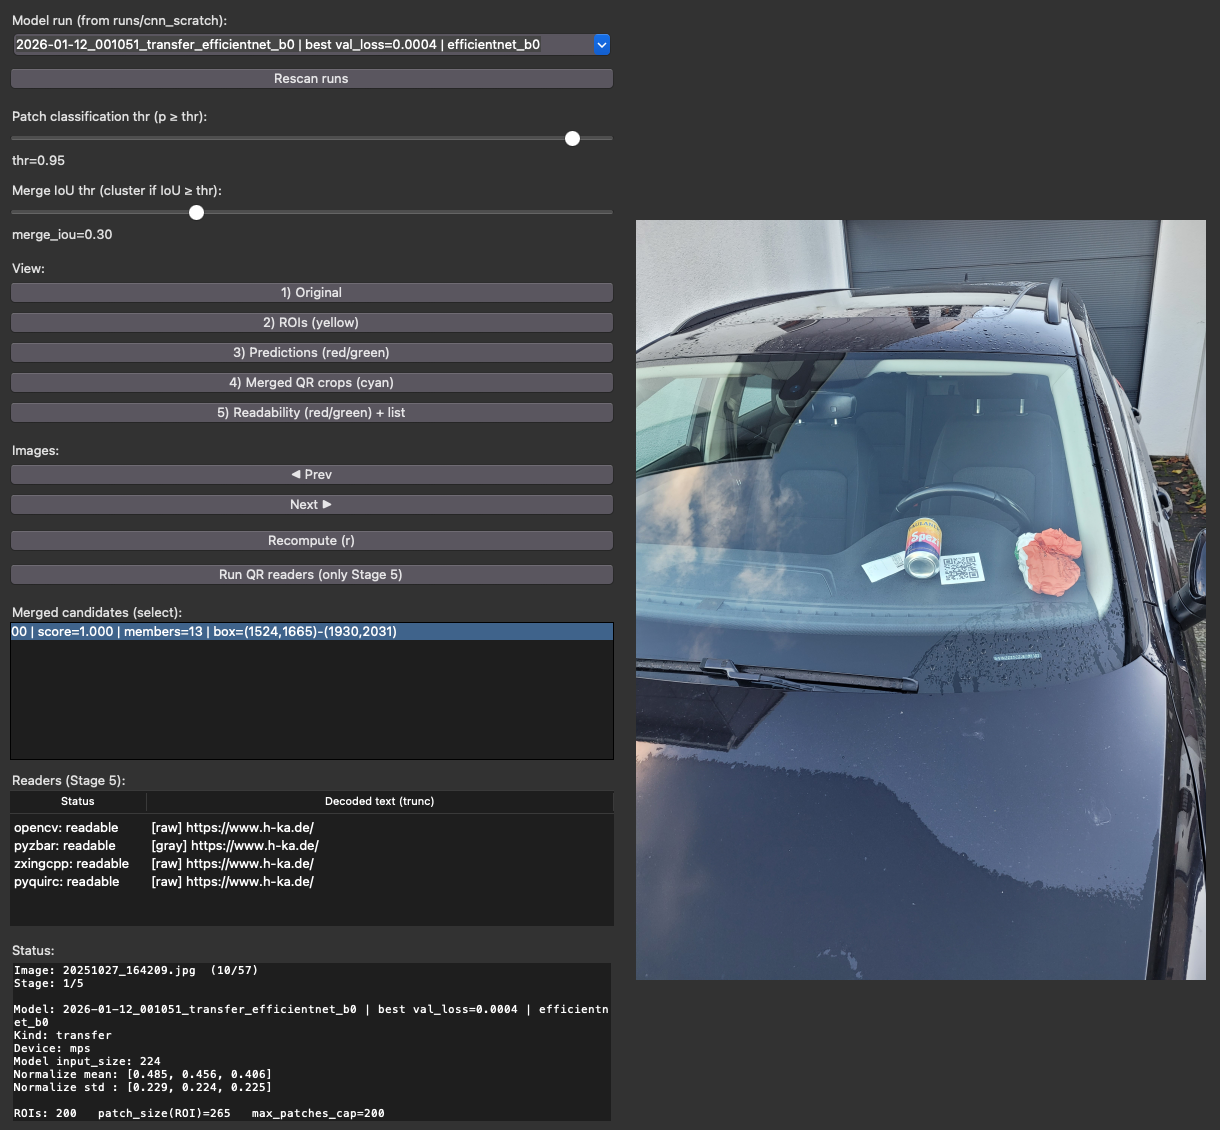
\includegraphics[width=\linewidth]{Figures/png/gui_view1_original.png}
        \caption*{(1) Original}
    \end{minipage}\hfill
    \begin{minipage}{0.49\linewidth}
        \centering
        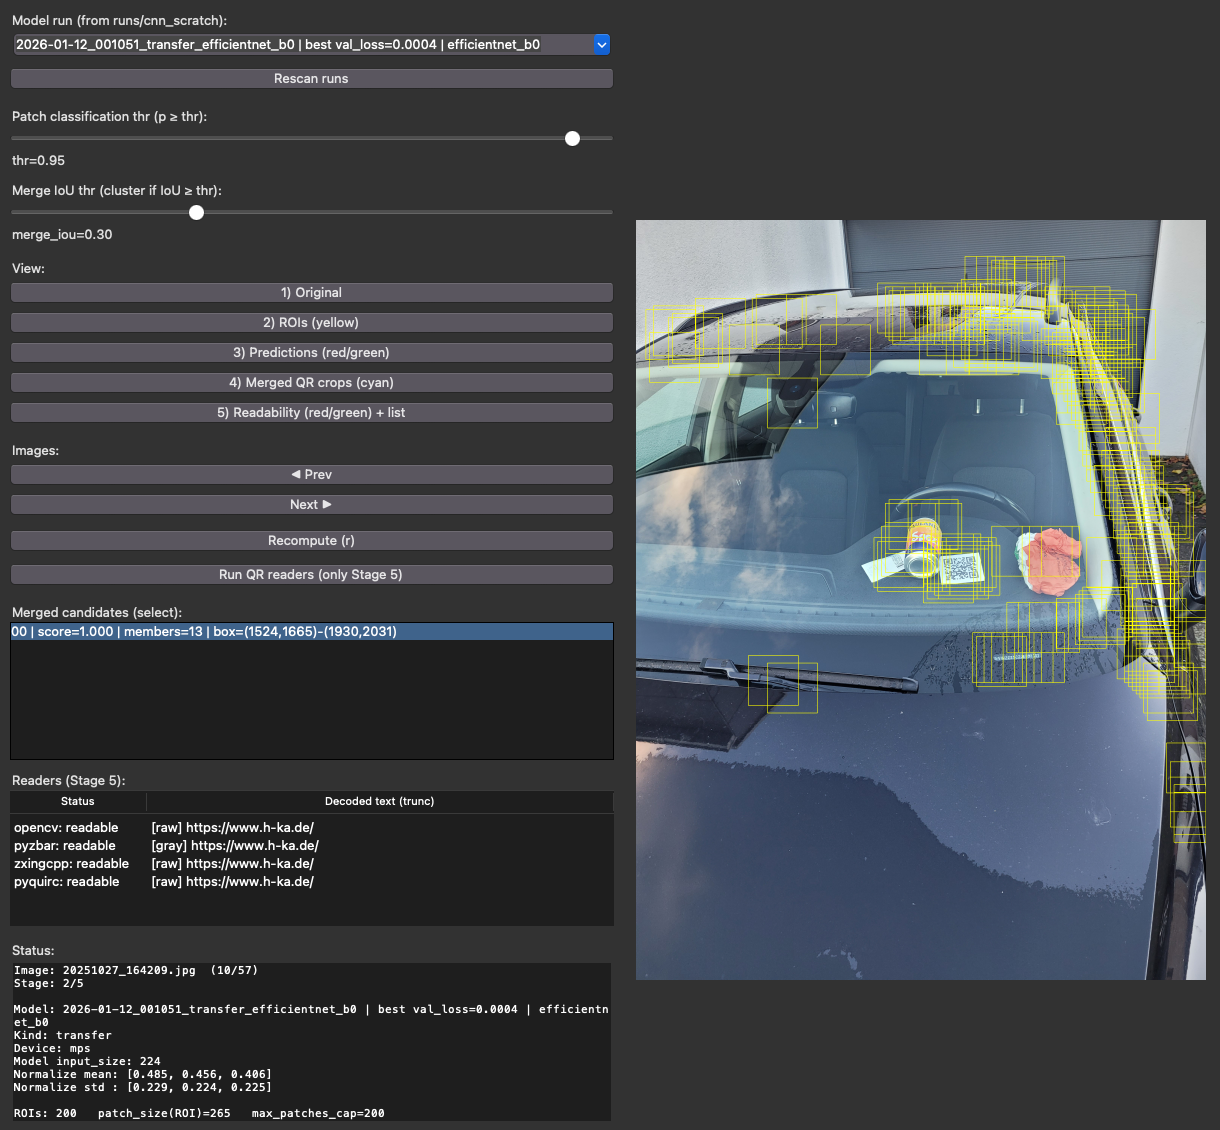
\includegraphics[width=\linewidth]{Figures/png/gui_view2_rois.png}
        \caption*{(2) ROIs (gelb)}
    \end{minipage}

    \vspace{0.6em}

    \begin{minipage}{0.49\linewidth}
        \centering
        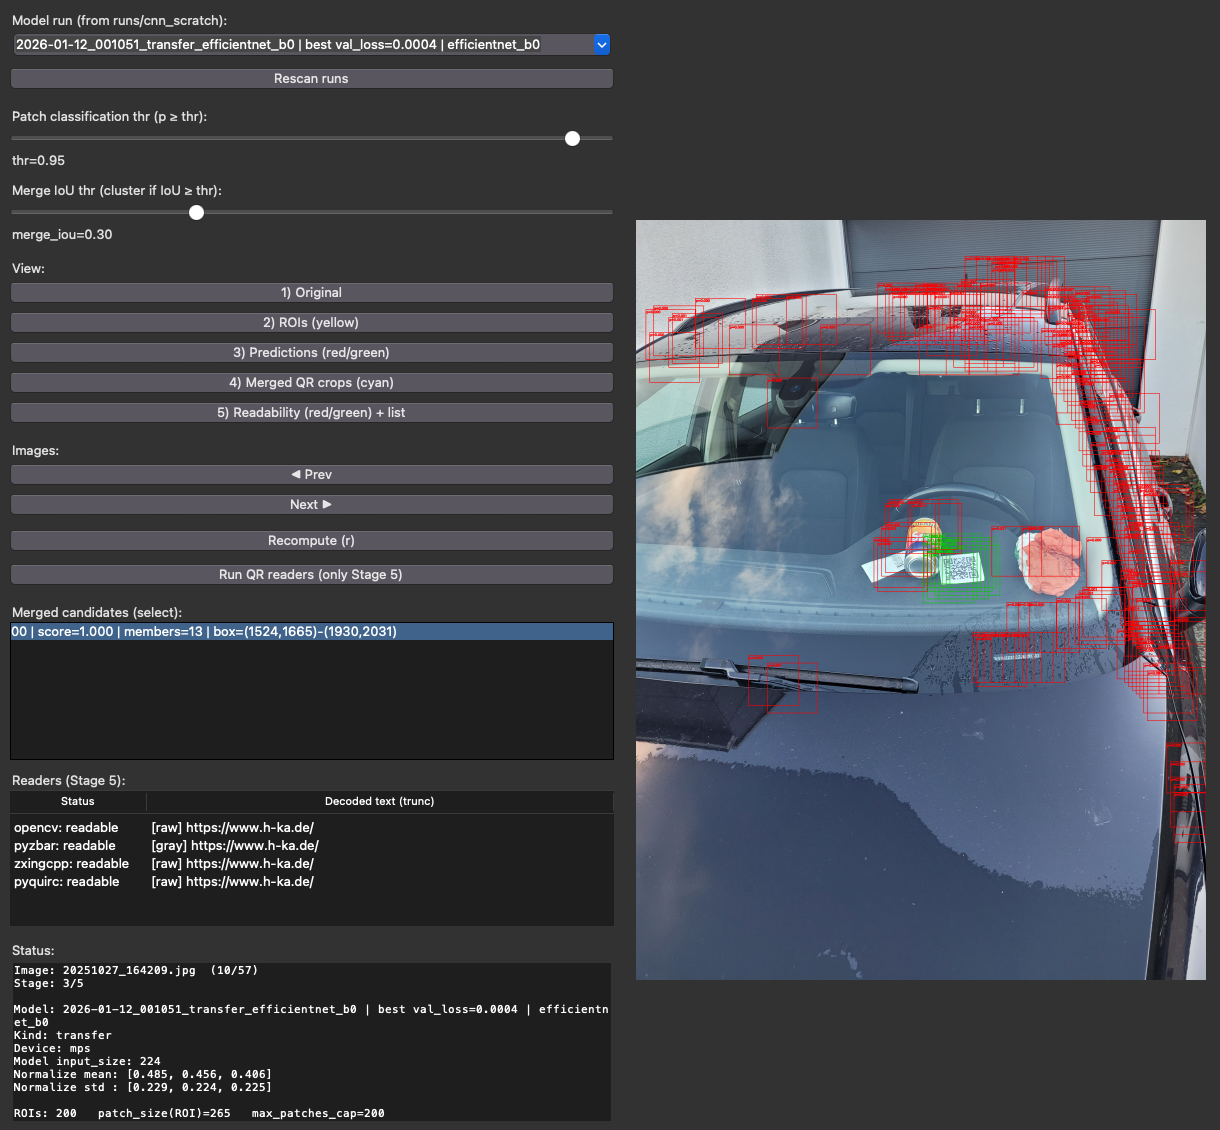
\includegraphics[width=\linewidth]{Figures/png/gui_view3_predictions.png}
        \caption*{(3) Predictions (rot/grün)}
    \end{minipage}\hfill
    \begin{minipage}{0.49\linewidth}
        \centering
        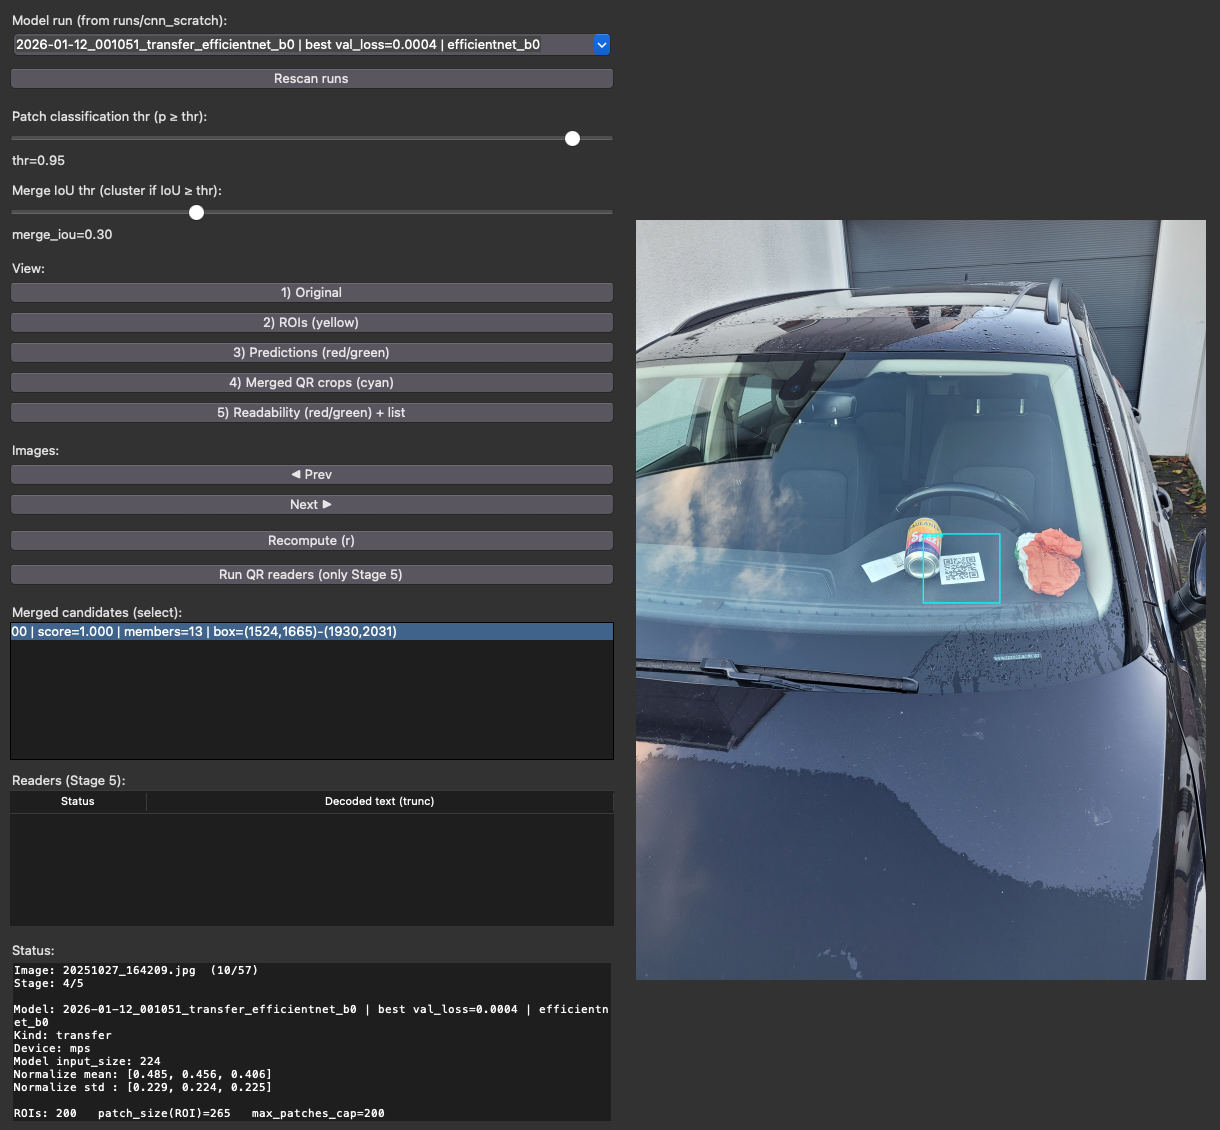
\includegraphics[width=\linewidth]{Figures/png/gui_view4_merged.png}
        \caption*{(4) Merged QR crops (cyan)}
    \end{minipage}

    \vspace{0.6em}

    \begin{minipage}{0.70\linewidth}
        \centering
        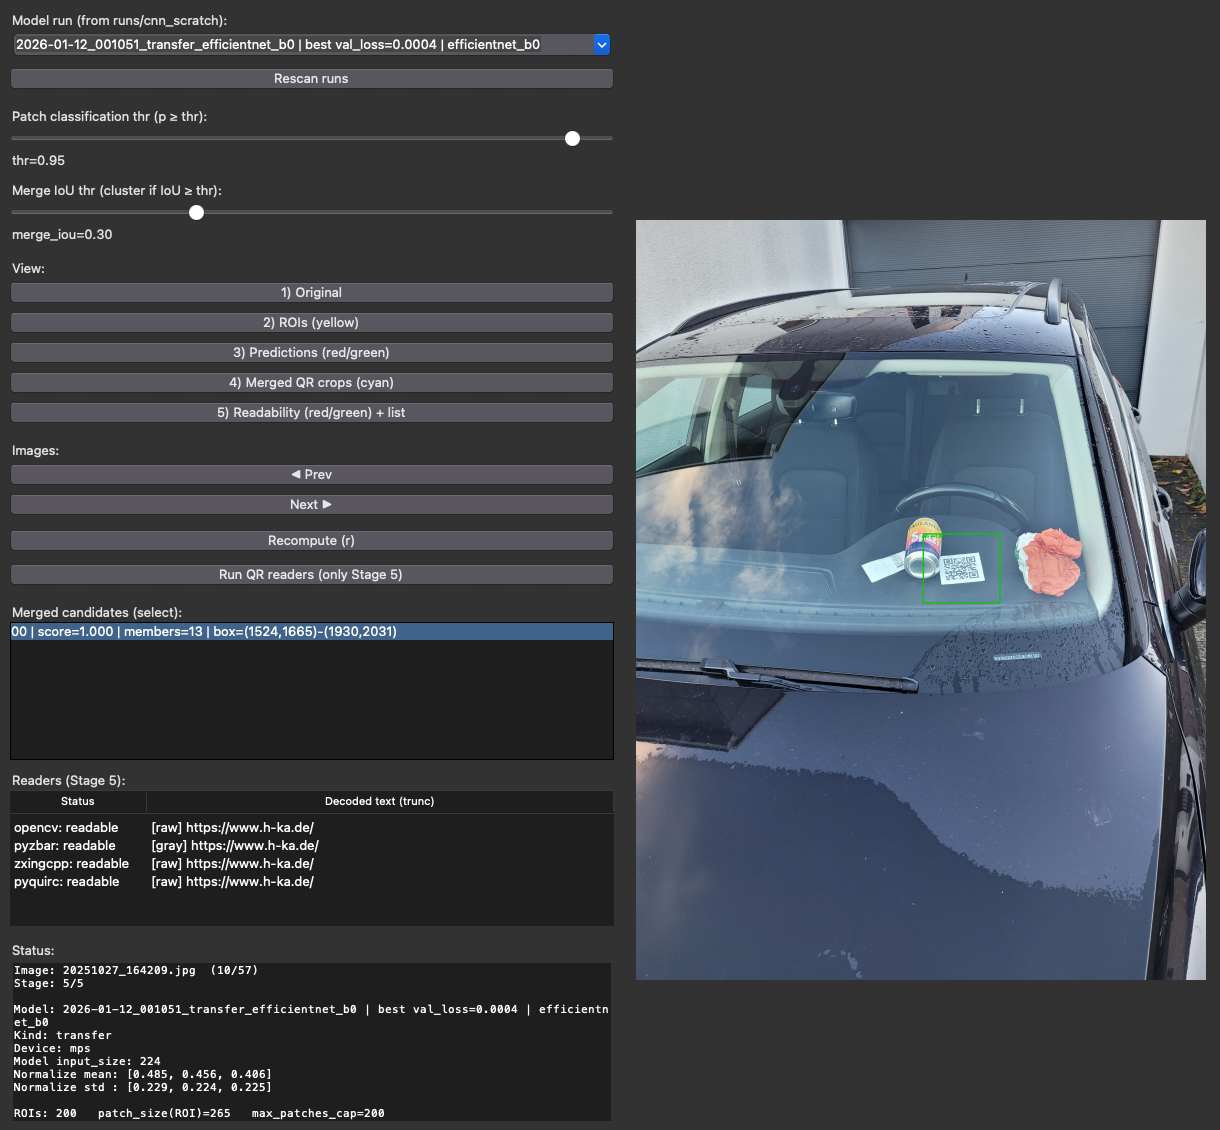
\includegraphics[width=\linewidth]{Figures/png/gui_view5_readability.png}
        \caption*{(5) Readability (rot/grün) + Reader-Liste}
    \end{minipage}

    \caption{Fünf Ansichten des Prediction-GUIs zur QR-Code-Lokalisierung und Lesbarkeitsprüfung (gleiches Bild, gleiche Modelleinstellungen).}
    \label{fig:gui_views}
\end{figure}


\section{Lesbarkeitsprüfung}
\label{sec:lesbarkeit}

\subsection{Motivation: Decoder sind inkonsistent}
\label{subsec:decoder_problem}

Nach dem Merging liegt pro Kandidat eine Box vor, die \glqq wahrscheinlich\grqq{} einen QR-Code enthält. Für die tatsächliche Nutzbarkeit ist jedoch entscheidend, ob der QR-Code auch \textbf{dekodierbar} ist. In der Praxis zeigte sich, dass einzelne QR-Decoder auf schwierigen Bildern (Reflexion, Nässe, Schaum, Bewegungsunschärfe, Kompressionsartefakte, Teilabdeckung) teils inkonsistent reagieren: Ein Decoder kann in einem Bild erfolgreich sein, während er im nächsten Bild trotz ähnlicher Situation scheitert.

Aus diesem Grund wurde eine \textbf{Multi-Reader-Strategie} implementiert: Mehrere Decoder laufen parallel, und sobald mindestens ein Decoder den QR-Code lesen kann, wird die Region als \textbf{lesbar} markiert (grüner Rahmen). Damit wird die Lesbarkeitsentscheidung deutlich stabiler als mit einem einzelnen Reader. :contentReference[oaicite:5]{index=5}

\subsection{Reader-Kaskade und Vorverarbeitungsvarianten}
\label{subsec:decoder_pipeline}

Im GUI werden folgende Reader genutzt (sofern installiert/verfügbar):
\begin{itemize}
    \item OpenCV \texttt{QRCodeDetector},
    \item \texttt{pyzbar},
    \item \texttt{zxingcpp},
    \item \texttt{pyquirc} (quirc).
\end{itemize}
Jeder Reader erhält nicht nur das rohe Crop, sondern mehrere einfache Vorverarbeitungsvarianten, um schwierige Fälle abzufangen:
\begin{itemize}
    \item \textbf{raw}: unverändertes Crop,
    \item \textbf{gray}: Graustufenvariante,
    \item \textbf{upscaled}: Vergrößerung kleiner Crops (Interpolation), falls die Region sehr klein ist,
    \item \textbf{adaptive threshold}: binarisierte Variante, die häufig bei Reflexionen oder ungleichmäßiger Beleuchtung hilft.
\end{itemize}
Der Reader versucht die Varianten der Reihe nach; sobald ein gültiger Text extrahiert wurde, gilt dieser Reader als erfolgreich. Die Ergebnisse werden im GUI als Liste angezeigt (Readername, Status, gekürzter Text und verwendete Variante). :contentReference[oaicite:6]{index=6}

\subsection{Kriterium: wann ist ein QR-Code lesbar?}
\label{subsec:lesbar_kriterium}

Ein gemergter Kandidat wird als \textbf{lesbar} klassifiziert, wenn mindestens einer der Reader einen nicht-leeren Decodetext liefert:
\[
\texttt{READABLE} \Leftrightarrow \exists\, r \in \{\text{Reader}\}:\ r(\text{Crop})\ \text{liefert Text}
\]
In diesem Fall wird die Kandidatenregion im Bild \textbf{grün} markiert; andernfalls \textbf{rot}. In der Praxis ergab sich, dass bestimmte Reader (z.\,B. \texttt{pyquirc} oder \texttt{zxingcpp}) in vielen Fällen robuster wirkten als OpenCV – jedoch nicht konstant in jedem Bild. Genau deshalb ist die Mehrfachausführung entscheidend: Sie erhöht die Wahrscheinlichkeit, dass zumindest ein Reader unter den jeweiligen Bildstörungen erfolgreich ist.

\subsection{Zwischenfazit}
\label{subsec:lesbarkeit_fazit}

Die Kombination aus (i) konservativem Patch-Threshold (\texttt{thr=0.95}), (ii) IoU-basiertem Merging (\texttt{merge\_iou=0.30}) und (iii) Multi-Reader-Decoding stellt eine robuste, gut interpretierbare Pipeline dar. Sie verbindet die gelernten CNN-Entscheidungen (QR vs. No-QR auf Patches) mit einer praktischen Nutzbarkeitsprüfung (dekodierbarer QR-Code) und ermöglicht über das GUI schnelle, nachvollziehbare Tests auf beliebigen Bildern.
